\documentclass[t, aspectratio=169, table]{beamer}

%%%%%%%%%%
%%% Packages
%%%%%%%%%%

\usepackage{xcolor}
\usepackage{hhline}
\usepackage{booktabs}
\usepackage{nicefrac}
\usepackage{tikz}
\usetikzlibrary{intersections}
\usetikzlibrary{calc}
\usetikzlibrary{quantikz2}
\usepackage{tcolorbox}
\tcbuselibrary{theorems}

\newtcbtheorem{cbox}{}{
  boxrule=0.15mm,
  colback=gray!15,
  % colbacktitle=gray!15,
  % coltitle=red!50!black,
  % fonttitle=\bfseries,
  coltext=red!40!black,
  detach title,
  % before upper={\tcbtitle},
  % separator sign none,
  % description delimiters={(}{). }
}{cbox}

\newcommand{\ketbra}[2]{\ensuremath{| #1 \rangle \langle #2 |}}
\newcommand{\ci}{\mathrm{i}}
\DeclarePairedDelimiter{\card}{\lvert}{\rvert}
\DeclarePairedDelimiter{\norm}{\lVert}{\rVert}
\DeclareMathOperator{\tr}{tr}
\newcommand{\cnot}{\mathit{CNOT}}

%%%%%%%%%%
%%% Sections
%%%%%%%%%%

\newif{\ifsectionPage}
\newcommand{\sectionPageDefault}{\global\sectionPagetrue}
\newcommand{\disableNextSectionPage}{\global\sectionPagefalse}
\sectionPageDefault{}
\AtBeginSection[]{%
  \ifsectionPage{}
    \frame{\sectionpage}
  \fi
  \sectionPageDefault{}}

%%%%%%%%%%
%%% Doc Info
%%%%%%%%%%

\newcommand{\email}[1]{\href{mailto:#1}{#1}}
\author[Luigi Soares \& Roberto Rosmaninho]{%
  Luigi Soares (\email{luigi.domenico@dcc.ufmg.br}) \\
  Roberto Rosmaninho (\email{robertogomes@dcc.ufmg.br})}
\institute[DCC/UFMG]{}
\date{03/07/2023}
\title[Jogos Mágicos Quânticos]{Jogos Mágicos Quânticos}

\usetheme{ufmg}

\begin{document}
\maketitle

\section{Quadrado Mágico}

\begin{frame}{Introdução ao Jogo}
  \begin{itemize}[<+->]
  \item Jogo cooperativo não-local
  \item Dois jogadores: Alice e Bob
  \item Um árbitro: Charlie
  \item Alice e Bob não podem se comunicar após o início
  \item A cada rodada:
    \begin{enumerate}[<+->]
    \item Charlie sorteia uma linha 0, 1 ou 2 de uma matriz \(3 \times 3\) e atribui à Alice
    \item Alice preenche as três células com \(+1\) ou \(-1\), de forma que o produto seja \(+1\)
    \item Charlie sorteia uma coluna 0, 1 ou 2 da matriz e atribui ao Bob
    \item Bob preenche as três células com \(+1\) ou \(-1\), de forma que o produto seja \(-1\)
    \item Alice e Bob vencem se respeitaram  e concordaram
      no valor da interseção
    \end{enumerate}
  \end{itemize}
\end{frame}

\begin{frame}{Exemplo 1 (Vitória)}
  \renewcommand{\arraystretch}{2}
  \vfill{}
  \begin{minipage}{0.45\textwidth}
    \begin{center}
      Alice \(\leftarrow 0\)
    \end{center}
    \[\begin{array}{|>{\quad}c<{\quad}|*{2}{>{\quad}c<{\quad}|}c}
        \hhline{---}
        +1 & \cellcolor{gray!50} -1 & -1 & \prod = +1
        \\ \hhline{---}
           & & &
        \\ \hhline{---}
           & & &
        \\ \hhline{---}
        \multicolumn{1}{c}{}
        & \multicolumn{1}{c}{}
        & \multicolumn{1}{c}{}
      \end{array}\]
  \end{minipage}
  \hfill{}
  \begin{minipage}{0.45\textwidth}
    \begin{center}
      Bob \(\leftarrow 1\)
    \end{center}
    \[\begin{array}{|>{\quad}c<{\quad}|*{2}{>{\quad}c<{\quad}|}}
        \hhline{---}
        \phantom{+1} & \cellcolor{gray!50}-1 & \phantom{-1}
        \\ \hhline{---}
           & +1 &
        \\ \hhline{---}
           & +1 &
        \\ \hhline{---}
        \multicolumn{1}{c}{}
        & \multicolumn{1}{c}{\prod = -1}
        & \multicolumn{1}{c}{}
      \end{array}\]
  \end{minipage}  
  \vfill{}
\end{frame}

\begin{frame}{Exemplo 2 (Derrota, Interseção)}
  \renewcommand{\arraystretch}{2}
  \vfill{}
  \begin{minipage}{0.45\textwidth}
    \begin{center}
      Alice \(\leftarrow 1\)
    \end{center}
    \[\begin{array}{|>{\quad}c<{\quad}|*{2}{>{\quad}c<{\quad}|}c}
        \hhline{---}
           & & &
        \\ \hhline{---}
        +1 & \cellcolor{red!80!black!55} -1 & -1 & \prod = +1
        \\ \hhline{---}
           & & &
        \\ \hhline{---}
        \multicolumn{1}{c}{}
        & \multicolumn{1}{c}{}
        & \multicolumn{1}{c}{}
      \end{array}\]
  \end{minipage}
  \hfill{}
  \begin{minipage}{0.45\textwidth}
    \begin{center}
      Bob \(\leftarrow 1\)
    \end{center}
    \[\begin{array}{|>{\quad}c<{\quad}|*{2}{>{\quad}c<{\quad}|}}
        \hhline{---}
        \phantom{+1} & -1 & \phantom{-1}
        \\ \hhline{---}
           & \cellcolor{red!80!black!55} +1 &
        \\ \hhline{---}
           & +1 &
        \\ \hhline{---}
        \multicolumn{1}{c}{}
        & \multicolumn{1}{c}{\prod = -1}
        & \multicolumn{1}{c}{}
      \end{array}\]
  \end{minipage}  
  \vfill{}
\end{frame}

\begin{frame}{Exemplo 3 (Derrota, Produto)}
  \renewcommand{\arraystretch}{2}
  \vfill{}
  \begin{minipage}{0.45\textwidth}
    \begin{center}
      Alice \(\leftarrow 1\)
    \end{center}
    \[\begin{array}{|>{\quad}c<{\quad}|*{2}{>{\quad}c<{\quad}|}c}
        \hhline{---}
           & & &
        \\ \hhline{---}
        +1 & \cellcolor{gray!50} +1 & -1 & \cellcolor{red!80!black!55}\prod = -1
        \\ \hhline{---}
           & & &
        \\ \hhline{---}
        \multicolumn{1}{c}{}
        & \multicolumn{1}{c}{}
        & \multicolumn{1}{c}{}
      \end{array}\]
  \end{minipage}
  \hfill{}
  \begin{minipage}{0.45\textwidth}
    \begin{center}
      Bob \(\leftarrow 1\)
    \end{center}
    \[\begin{array}{|>{\quad}c<{\quad}|*{2}{>{\quad}c<{\quad}|}}
        \hhline{---}
        \phantom{+1} & -1 & \phantom{-1}
        \\ \hhline{---}
           & \cellcolor{gray!50} +1 &
        \\ \hhline{---}
           & +1 &
        \\ \hhline{---}
        \multicolumn{1}{c}{}
        & \multicolumn{1}{c}{\prod = -1}
        & \multicolumn{1}{c}{}
      \end{array}\]
  \end{minipage}  
  \vfill{}
\end{frame}

\begin{frame}{Estratégia Clássica (Determinística)}
  \begin{itemize}[<+->]
  \item Alice e Bob não podem se comunicar \emph{durante} o jogo, mas
    podem \emph{antes}
    
  \item Uma estratégia determinística consiste em 
    preparar matrizes pré-definidas
    
  \item<only@7-> É impossível vencer com 100\% de chance toda rodada
    
  \item<only@9-> A melhor estratégia determinística vence com probabilidade \(\nicefrac{8}{9}\)
  \end{itemize}

  \only<3-6>{
    \renewcommand{\arraystretch}{2}
    \vfill{}
    \begin{minipage}{0.45\textwidth}
      \begin{center}
        Alice
        \[\begin{array}{|>{\quad\columncolor{gray!50}}c<{\quad}|*{2}{>{\quad}c<{\quad}|}}
            \hhline{---}
            -1 & \onslide<4->{\only<5->{\cellcolor{gray!50}}-1} & \onslide<4->{\only<6->{\cellcolor{red!80!black!55}}+1}
            \\ \hhline{---}
            -1 & \onslide<4->{\only<5->{\cellcolor{gray!50}}-1} & \onslide<4->{\only<6->{\cellcolor{gray!50}}+1}
            \\ \hhline{---}
            -1 & \onslide<4->{\only<5->{\cellcolor{gray!50}}-1} & \onslide<4->{\only<6->{\cellcolor{gray!50}}+1}
            \\ \hhline{---}
          \end{array}\]
      \end{center}
    \end{minipage}
    \hfill{}
    \begin{minipage}{0.45\textwidth}
      \begin{center}
        Bob
        \[\begin{array}{|>{\quad\columncolor{gray!50}}c<{\quad}|*{2}{>{\quad}c<{\quad}|}}
            \hhline{---}
            -1 & \onslide<5->{\only<5->{\cellcolor{gray!50}}-1} & \onslide<6->{\only<6->{\cellcolor{red!80!black!55}}-1}
            \\ \hhline{---}
            -1 & \only<5->{\cellcolor{gray!50}-1} & \only<6->{\cellcolor{gray!50}+1}
            \\ \hhline{---}
            -1 & \only<5->{\cellcolor{gray!50}-1} & \only<6->{\cellcolor{gray!50}+1}
            \\ \hhline{---}
          \end{array}\]
      \end{center}
    \end{minipage}  
    \vfill{}
  }

  \only<8>{
    \[\begin{aligned}
        m_{0,0}\, m_{0,1}\, m_{0,2} &= +1 \\
        m_{1,0}\, m_{1,1}\, m_{1,2} &= +1 \\
        m_{2,0}\, m_{2,1}\, m_{2,2} &= +1 \\
        m_{0,0}\, m_{1,0}\, m_{2,0} &= -1 \\
        m_{0,1}\, m_{1,1}\, m_{2,1} &= -1 \\
        m_{0,2}\, m_{1,2}\, m_{2,2} &= -1 \\
        \midrule
        +1 &\neq -1
      \end{aligned}\]
  }
\end{frame}

\begin{frame}{Estratégia Clássica (Probabilística)}
  \begin{itemize}[<+->]
  \item Alice e Bob jogam uma moeda para decidir o valor de cada célula
    
  \item Isto é equivalente a cada um deles sortear uma
    dentre todas as possíveis matrizes
    
  \item A combinação das duas matrizes sorteadas é uma estratégia determinística
    
  \item Ou seja, qualquer estratégia probabilística é limitada pela
    melhor estratégia determinística. Logo, a chance de sucesso
    clássico é no máximo \(\nicefrac{8}{9}\)
  \end{itemize}
\end{frame}

\begin{frame}{Estratégia Quântica}
  \begin{itemize}[<only@+-5>]
  \item E se Alice e Bob puderem carregar qubits?
    
  \item Existe uma estratégia quântica que os permite vencer qualquer
    rodada

  \item Alice e Bob compartilham qubits emaranhados
    \[
      \ket{\psi} = \frac{1}{2}\left(
        \ket{00}_{A} \otimes \ket{00}_{B} + \ket{01}_{A} \otimes \ket{01}_{B} +
        \ket{10}_{A} \otimes \ket{10}_{B} + \ket{11}_{A} \otimes \ket{11}_{B}
      \right)
    \]
    
  \item Ao receber uma linha/coluna, eles medem seus qubits
    
  \item  O resultado de cada medição é o valor de cada célula
  \end{itemize}

  \only<+->{
    \renewcommand{\arraystretch}{2}
    \centering
    \[\begin{array}{|*{3}{>{\quad}c<{\quad}|}c}
        \hhline{---~}
        +I \otimes Z & +Z \otimes I & +Z \otimes Z & \onslide<.(1)->{\color{green!50!black}+I}
        \\ \hhline{---~}
        +X \otimes I & +I \otimes X & +X \otimes X & \onslide<.(1)->{\color{green!50!black}+I}
        \\ \hhline{---~}
        -X \otimes Z & -Z \otimes X & +Y \otimes Y & \onslide<.(1)->{\color{green!50!black}+I}
        \\ \hhline{---~}
        \multicolumn{1}{c}{\onslide<.(1)->{\color{red!50!black}-I}} &
        \multicolumn{1}{c}{\onslide<.(1)->{\color{red!50!black}-I}} &
        \multicolumn{1}{c}{\onslide<.(1)->{\color{red!50!black}-I}} &
      \end{array}\]
  }
\end{frame}

\begin{frame}{Exemplo 4}
  \begin{enumerate}
  \item<only@1-3> Alice recebe a linha 0 e mede seu segundo qubit com
    \(Z\). Suponha que ela tenha observado \(+1\). Ela atribui \(+1\)
    à primeira celula e o estado inicial \(\ket{\psi}\) colapsa para
    \[
      \ket{\psi_{A1}} = \frac{1}{\sqrt{2}} (\ket{0000} + \ket{1010})
    \]
  \item<only@2-3> Em seguida, Alice mede seu primeiro qubit com \(Z\). Suponha que
    ela tenha observado \(-1\). Ela atribui \(-1\) à segunda célula e o estado
    colapsa para
    \[
      \ket{\psi_{A2}} = \ket{1010}
    \]
  \item<only@3> Para a terceira célula, ela mede seus dois qubits com \(Z \otimes Z\).
    O único resultado possível é \(-1\) e o estado não se altera:
    \(
      \ket{\psi_{A3}} = \ket{\psi_{A2}}.
    \)
    
  \item<only@4-> Suponha que Bob tenha recebido a coluna 1. Para a primeira
    célula, ele mede seu primeiro qubit com \(Z\). Ele observa \(-1\)
    (igual Alice) com probabilidade 1, e
    \[
      \ket{\psi_{B1}} = \ket{\psi_{A3}} = \ket{1010}
    \]
    
  \item<only@5-> Em seguida, Bob mede seu segundo qubit com \(X\).
    Suponha que ele observe \(+1\). Então, o estado colapsa para
    \[
      \ket{\psi_{B2}} = \frac{1}{\sqrt{2}} (\ket{1010} + \ket{1011})
    \]

  \item<only@6-> Para a terceira célula, ele mede ambos os qubits com
    \(-Z \otimes X\).  O único resultado possível é \(+1\), o que
    satisfaz a restrição sobre o produto da coluna.
  \end{enumerate}
\end{frame}

\begin{frame}{Lema 1: Produto das Linhas e Colunas}
  \begin{cbox}{}{msquare-quantum-prod}
    Seja \(M_{i, j}\) o observável na célula \((i, j)\) da estratégia
    quântica, segue que, para toda linha \(i\),
    \(\prod_{j} \operatorname{Out}(M_{i, j}) = +1\), e, para toda
    coluna \(j\), \(\prod_{i} \operatorname{Out}(M_{i, j}) = -1\).
  \end{cbox}

  \begin{itemize}[<+(1)->]
  \item Note que, em qualquer linha e coluna, os três
    observáveis comutam entre si
    
  \item Ou seja, é possível encontrar uma base de autovetores em comum, que
    diagonaliza os três. Para toda linha \(i\) (equiv. coluna \(j\)),
    \begin{align*}
      M_{i,0} M_{i,1} M_{i,2} &= (P_{i} \Lambda_{i, 0}P^{-1}) (P_{i} \Lambda_{i, 1}P^{-1}) (P_{i} \Lambda_{i, 2}P_{i}^{-1}) \\
      &= P_{i} (\Lambda_{i, 0} \Lambda_{i, 1} \Lambda_{i, 2})P_{i}^{-1} \\
      &= P_{i} \Lambda_{i} P_{i}^{-1}
    \end{align*}
    
  \item Cada entrada de \(\Lambda_{i}\) é o produto dos autovalores p/ mesmo autovetor
  \end{itemize}
\end{frame}

\begin{frame}{Lema 1: Produto das Linhas e Colunas}
  \begin{itemize}[<+->]
  \item Os autovalores são sempre \(+1\) e \(-1\)
    
  \item Tem sempre dois autovetores em comum para cada autoespaço
    
  \item O que isso significa é que a primeira medição de qualquer
    linha/coluna resulta em um autovalor \(\lambda\) e colapsa para uma
    combinação de dois autovetores \(\ket{\lambda}_{0}\) e
    \(\ket{\lambda}_{1}\)
    
  \item A segunda medição, então, colapsa para \(\ket{\lambda}_{0}\)
    ou \(\ket{\lambda}_{1}\), e fixa o estado

  \item Logo, as medições irão resultar nos autovalores correspondentes
    a \(\ket{\lambda}_{0}\)  ou \(\ket{\lambda}_{1}\)

  \item O produto das três medições é uma das entradas de \(\Lambda_{i}\)
    
  \item Mas, para toda linha \(i\), temos
    \(P_{i} \Lambda_{i} P_{i}^{-1} = I\). Logo, \(\Lambda_{i} = I\) e o
    produto das três medições é \(+1\) sempre. Para toda coluna \(j\),
    \(P_{j} \Lambda_{j} P_{j}^{-1} = -I\) e \(\Lambda_{j} = -I\) 
  \end{itemize}

  \only<.->{\qed}
\end{frame}

\begin{frame}{Lema 1: Produto das Linhas e Colunas}
  \begin{itemize}[<+->]
  \item Para a primeira linha, os autovetores em comum são
    \(\ket{00}, \ket{01}, \ket{10}\) e \(\ket{11}\)

  \item Para a primeira célula \(I \otimes Z\), temos \(\ket{00}\) e
    \(\ket{10}\) no autoespaço do \(+1\)
    
  \item Ao observar \(+1\), o estado colapsa para uma combinação dos dois, vide Exemplo 4:
    \[
      \frac{1}{2} (\ket{0000} + \ket{0101} + \ket{1010} + \ket{1111})
      \mapsto
      \frac{1}{\sqrt{2}} (\ket{0000} + \ket{1010})
    \]

  \item Para a segunda célula \(Z \otimes I\), o autovalor de \(\ket{00}\) é
    \(+1\) e o de \(\ket{10}\) é \(-1\)

  \item Ao observar \(-1\), o estado colapsa para o autovetor \(\ket{10}\),
    vide Exemplo 4:
    \[
      \frac{1}{\sqrt{2}} (\ket{0000} + \ket{1010})
      \mapsto
      \ket{1010}
    \]  \end{itemize}
\end{frame}

\begin{frame}{Lema 2: Interseção}
  \begin{cbox}{}{msquare-quantum-inters}
    Para qualquer linha \(i\) atribuída a Alice e
    coluna \(j\) atribuída ao Bob, o valor assinalado
    por ambos à célula \((i, j)\) é sempre o mesmo.
  \end{cbox}

  \begin{itemize}[<+(1)->]
  \item Independente da linha atribuída a Alice, o estado final dos qubits dela
    é sempre um dos autovetores em comum para aquela linha
    
  \item Se Alice repetir qualquer medição, o resultado é o mesmo que o anterior
    
  \item Mas, este estado é uma combinação de um dos autoespaços de
    Bob na interseção

  \item Além disso, o estado inicial é simétrico e, a cada medição, a simetria se mantém
    
  \item Logo, se Bob mede os qubits dele com os mesmos observáveis que Alice, ele
    observa o mesmo resultado
  \end{itemize}
  
  \only<.(1)->{\qed}
\end{frame}

\begin{frame}{Lema 2: Interseção}
  \begin{itemize}[<+->]
  \item Para a segunda linha, o estado de Alice colapsa para
    \((\nicefrac{1}{2}) (\ket{00} + \ket{01} + \ket{10} + \ket{11})\),
    \((\nicefrac{1}{2}) (\ket{00} - \ket{01} + \ket{10} - \ket{11})\),
    \((\nicefrac{1}{2}) (\ket{00} - \ket{01} - \ket{10} + \ket{11})\) ou
    \((\nicefrac{1}{2}) (\ket{00} + \ket{01} - \ket{10} - \ket{11})\)

  \item Suponha que tenha sido \((\nicefrac{1}{2}) (\ket{00} - \ket{01} - \ket{10} + \ket{11})\)

  \item Então, Alice recebeu \(-1\), \(-1\) e \(+1\)

  \item Após a primeira medição, o estado colapsa para
    {
      \small
      \begin{align*}
        &\frac{1}{2\sqrt{2}} \Bigl(
          (\ket{00} - \ket{10}) \ket{00} +
          (\ket{01} - \ket{11}) \ket{01} +
          (\ket{10} - \ket{00}) \ket{10} +
          (\ket{11} - \ket{01}) \ket{11}
          \Bigr) \\
        \equiv\;
        & \frac{1}{2\sqrt{2}} \Bigl(
          \ket{00} (\ket{00} - \ket{10}) +
          \ket{01} (\ket{01} - \ket{11}) +
          \ket{10} (\ket{10} - \ket{00}) +
          \ket{11} (\ket{11} - \ket{01})
          \Bigr)
      \end{align*}
    }
  \end{itemize}
\end{frame}

\begin{frame}{Lema 2: Interseção}
  \begin{itemize}[<+->]
  \item Após a segunda medição, o estado colapsa (e fixa) para
    {
      \small
      \begin{alignat*}{2}
        &\frac{1}{4} \Bigl(
        &&(\ket{00} - \ket{01} - \ket{10} + \ket{11}) \ket{00} -
           (\ket{00} - \ket{01} - \ket{10} + \ket{11}) \ket{01} - \nonumber \\
        & &&(\ket{00} - \ket{01} - \ket{10} + \ket{11}) \ket{10} +
             (\ket{00} - \ket{01} - \ket{10} + \ket{11}) \ket{11}
             \Bigr) \nonumber \\
        \equiv\;
        & \frac{1}{4} \Bigl(
        &&\ket{00} (\ket{00} - \ket{01} - \ket{10} + \ket{11}) -
           \ket{01} (\ket{00} - \ket{01} - \ket{10} + \ket{11}) - \nonumber \\
        & &&\ket{10} (\ket{00} - \ket{01} - \ket{10} + \ket{11}) +
             \ket{11} (\ket{00} - \ket{01} - \ket{10} + \ket{11})
             \Bigr)
      \end{alignat*}
    }
    
  \item Logo, para qualquer coluna que Bob receba, ao fazer uma
    medição igual a que Alice fez na interseção, ele obterá a mesma
    resposta que Alice
  \end{itemize}
\end{frame}

\begin{frame}{Teorema 1: O Jogo do Quadrado Mágico É Vencível}
  \begin{cbox}{}{thm:msquare}
    Existe uma estratégia quântica para o jogo do quadrado mágico de Mermin-Peres,
    que consiste em Alice e Bob compartilharem qubits emaranhados \emph{antes} do
    início do jogo, que vence sistematicamente todos as rodadas.
  \end{cbox}
\end{frame}

\section{Caracterizando Jogos Mágicos}

\begin{frame}{Modificando o Formato}
  \begin{itemize} [<+->]
  \item O que será que acontece se mudarmos o formato do jogo?
  \item E se, ao invés de um quadrado, fosse um pentagrama?
  \item<only@3-> Note que a representação foi em formato de grafo
  \item<only@4-> Podemos redesenhar o quadrado mágico como um grafo também
  \item<only@6-> Será que existe alguma caracterização deste tipo de jogo?
  \end{itemize}

  \only<2>{
    \vfill{}
    \begin{center}
      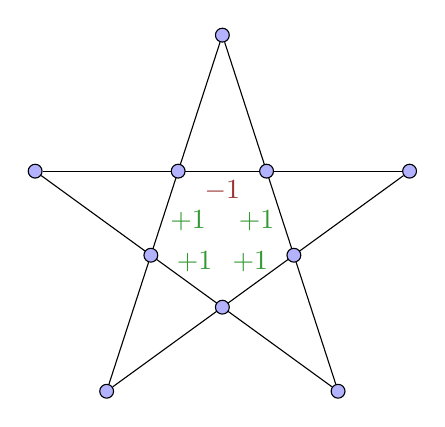
\begin{tikzpicture}[vertex/.style={circle, thin, fill=blue!30, draw, inner sep=0, minimum size=5pt}]
        \foreach \c [evaluate=\c as \ang using {18 + 72*\c}] in {0, 1, 2, 3, 4} {
          \node [vertex] (\c) at (\ang:25mm) {};
        }

        \draw [name path=0--2] (0) -- (2);
        \draw [name path=0--3] (0) -- (3);
        \draw [name path=1--3] (1) -- (3);
        \draw [name path=1--4] (1) -- (4);
        \draw [name path=2--4] (2) -- (4);

        \node [vertex] (01) at (intersection of 0--2 and 1--4) {};
        \node [vertex] (04) at (intersection of 0--3 and 1--4) {};
        \node [vertex] (12) at (intersection of 1--3 and 0--2) {};
        \node [vertex] (23) at (intersection of 1--3 and 2--4) {};
        \node [vertex] (34) at (intersection of 0--3 and 2--4) {};
        
        \node [text=red!50!black!80] (label0--2) at ($(01)!0.5!(12) - (0, 0.25)$) {\(-1\)};
        \node [text=green!50!black!80] (label1--4) at ($(01)!0.5!(04) + (-0.3, -0.1)$) {\(+1\)};
        \node [text=green!50!black!80] (label0--3) at ($(04)!0.5!(34) + (-0.1, 0.25)$) {\(+1\)};
        \node [text=green!50!black!80] (label2--4) at ($(23)!0.5!(34) + (+0.1, 0.25)$) {\(+1\)};
        \node [text=green!50!black!80] (label1--3) at ($(12)!0.5!(23) + (+0.3, -0.1)$) {\(+1\)};
        
        % (intersection cs:first line={(0) -- (2)}, second line={(1) -- (4)})
        % \node [vertex] (01) {}
        % (0) edge (2) edge (3)
        % (1) edge (3) edge (4)
        % (2) edge (4)
        % ;
        % % Triângulo de cima
        % \node (0) [vertex] at (0, +1) {};
        % \node (1) [vertex] at (-0.9, -1) {};
        % \node (2) [vertex] at (+0.9, -1) {};
        % \node (label0) [text=red!50!black!80] at (0, -1.25) {\(-I\)};
        
        % % Triângulo da esquerda
        % \node (3) [vertex] at (-2.75, -1) {};
        % \node (4) [vertex] at (-1.3, -2) {};
        % \node (label1) [text=green!50!black!80] at (-0.8, -1.5) {\(+I\)};

        % % Triângulo da direita
        % \node (5) [vertex] at (+2.75, -1) {};
        % \node (6) [vertex] at (+1.3, -2) {};
        % \node (label1) [text=green!50!black!80] at (+0.8, -1.5) {\(+I\)};

        % % Fechar pentágono
        % \node (7) [vertex] at (0, -2.75) {};
        % \node (label2) [text=green!50!black!80] at (+0.5, -2.1) {\(+I\)};
        % \node (label3) [text=green!50!black!80] at (-0.5, -2.1) {\(+I\)};

        % % Triângulo baixo esquerda
        % \node (8) [vertex] at (-1.9, -3.5) {};
        
        % % Triângulo baixo direita
        % \node (9) [vertex] at (+1.9, -3.5) {};
        
        % \path[]
        % (0) edge (1) edge (2)
        % (1) edge (2) edge (3) edge (4)
        % (2) edge (5) edge (6)
        % (3) edge (4)
        % (4) edge (7) edge (8)
        % (5) edge (6)
        % (6) edge (7) edge (9)
        % (7) edge (8) edge (9)
        % ;
      \end{tikzpicture}
    \end{center}
    \vfill{}
  }

  \only<5>{
    \vfill{}
    \begin{center}
      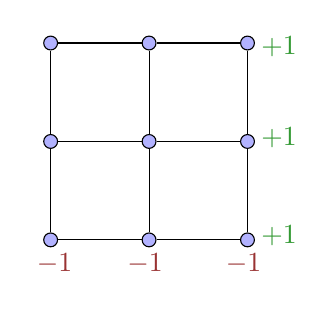
\begin{tikzpicture}[vertex/.style={circle, thin, fill=blue!30, draw, inner sep=0, minimum size=5pt}]
        % \node (phantom) [
        % label=above right:{\phantom{\(-X \otimes Z\)}},
        % label=below right:{\phantom{\(-X \otimes Z\)}}
        % ] at (1.5, -3) {};
        
        \node (00) [vertex,
        % label=above left:{\(I \otimes Z\)}
        ] at (-1.25, 0) {};
        \node (01) [vertex,
        % label=above left:{\(Z \otimes I\)}
        ] at (0,  0) {};
        \node (02) [vertex,
        % label=above left:{\(Z \otimes X\)}
        ] at (1.25,  0) {};

        \node (10) [vertex,
        % label=above left:{\(X \otimes I\)}
        ] at (-1.25, -1.25) {};
        \node (11) [vertex,
        % label=above left:{\(I \otimes X\)}
        ] at (0,  -1.25) {};
        \node (12) [vertex,
        % label=above left:{\(X \otimes X\)}
        ] at (1.25,  -1.25) {};

        \node (20) [vertex,
        % label=above left:{\(-X \otimes Z\)}
        ] at (-1.25, -2.5) {};
        \node (21) [vertex,
        % label=above left:{\(-Z \otimes X\)}
        ] at (0,  -2.5) {};
        \node (22) [vertex,
        % label=above left:{\(Y \otimes Y\)}
        ] at (1.25, -2.5) {};
        
        \only<.(1)->{\node (r0) [text=green!50!black!80] at (1.65, -0.05) {\(+1\)};}
        \only<.(1)->{\node (r1) [text=green!50!black!80] at (1.65, -1.20) {\(+1\)};}
        \only<.(1)->{\node (r2) [text=green!50!black!80] at (1.65, -2.45) {\(+1\)};}
        
        \only<.(1)->{\node (c0) [text=red!50!black!80] at (-1.2, -2.8) {\(-1\)};}
        \only<.(1)->{\node (c1) [text=red!50!black!80] at (-0.05, -2.8) {\(-1\)};}
        \only<.(1)->{\node (c2) [text=red!50!black!80] at (1.2, -2.8) {\(-1\)};}

        \path[]
        (00) edge (01) edge (10)
        (01) edge (02) edge (11)
        (02) edge (12)
        
        (10) edge (11) edge (20)
        (11) edge (12) edge (21)
        (12) edge (22)

        (20) edge (21)
        (21) edge (22)
        ;
      \end{tikzpicture}
    \end{center}
    \vfill{}
  }
\end{frame}

\begin{frame}{Definição 1 (Arranjo)}
  \begin{cbox}{}{arranjo}
    Um arranjo \(A = (V, E, \ell)\) é um hipergrafo conexo tal que
    cada vértice do conjunto \(V\) está exatamente em duas
    hiperarestas do conjunto \(E\) (\emph{conexo} significa que o
    hipergrafo não pode ser dividido em dois sub-hipergrafos
    disjuntos). O arranjo também inclui uma rotulação
    \(\ell\colon E \mapsto \{+1, -1\}\). 
  \end{cbox}

  \stepcounter{beamerpauses}
  \begin{itemize}[<+->]
  \item O quadrado mágico e o pentagrama são exemplos de arranjos
  \item Cada linha que passa por 3 vértices do quadrado é uma hiperaresta
  \item Cada linha que passa por 4 vértices do pentragrama é uma hiperaresta
  \end{itemize}
\end{frame}

\begin{frame}{Definição 2 (Realização Clássica)}
  \begin{cbox}{}{real-class}
    Uma realização clássica de um arranjo \(A = (V, E, \ell)\) é
    uma rotulação dos vértices \(c\colon V \mapsto \{+1, -1\}\)
    tal que, para cada \(e \in E\),
    % o produto dos rótulos de cada vértice em uma hiperaresta
    % é igual ao rótulo daquela hiperaresta:
    \(
      \prod_{v \in e} c(v) = \ell(e).
      % , \text{ para cada } e \in E.
    \)
  \end{cbox}

  \stepcounter{beamerpauses}
  \begin{itemize}[<+->]
  \item Por exemplo, considere uma versão \(2 \times 2\) do quadrado mágico, com
    \begin{align*}
      \ell(e_{t}) = \ell(e_{r}) &= +1 \text{ e } \\
      \ell(e_{b}) = \ell(e_{l}) &= -1 
    \end{align*}
    
  \item Uma realização clássica válida é
    \begin{align*}
      c(v_{00}) &= c(v_{01}) = c(v_{11}) = +1 \text{ e} \\
      c(v_{10}) &= -1
    \end{align*}
  \end{itemize}
  
  \onslide<2->{
    \begin{center}
      \begin{tikzpicture}[
        overlay, xshift=5cm, yshift=3.5cm,
        vertex/.style={circle, thin, fill=blue!30, draw, inner sep=0, minimum size=5pt}
        ]
        \node (00) [vertex] at (0, 0) {};
        \node (01) [vertex] at (1, 0) {};
        \node (10) [vertex] at (0, -1) {};
        \node (11) [vertex] at (1, -1) {};

        \node (et) [text=green!50!black!80] at (1.35, 0) {\(+1\)};
        \node (et) [text=green!50!black!80] at (0.9, -1.35) {\(+1\)};
        \node (et) [text=red!50!black!80] at (1.35, -0.9) {\(-1\)};
        \node (et) [text=red!50!black!80] at (-0.1, -1.35) {\(-1\)};

        \path[]
        (00) edge (01) edge (10)
        (01) edge (11)
        (10) edge (11)
        ;
      \end{tikzpicture}
    \end{center}
  }
\end{frame}

\begin{frame}{Definição 3 (Realização Quântica)}
  \begin{cbox}{}{real-quant}
    Uma realização quântica de um arranjo \(A = (V, E, \ell)\) é
    uma rotulação de vértices
    \(c\colon V \mapsto \operatorname{GL}(\mathcal{H})\), que
    mapeia cada vértice para um observável \(M\), tal que

    \begin{itemize}[<+(1)->]
    \color{red!40!black}
    \item \(M = M^{*}\) e \(M^{2} = I\), ou equivalentemente,
      \(M\) possui autovalores \(+1\) e \(-1\)

    \item Observáveis assinalados aos vértices de uma hiperaresta
      comutam entre si

    \item Para cada hiperaresta \(e \in E\), \(\prod_{v \in e} c(v) = \ell(e) I\)
    \end{itemize}
  \end{cbox}

  \begin{itemize}[<+(1)->]
  \item Uma realização clássica é simplesmente uma realização quântica com \(\mathcal{H} = \mathbb{R}\)
    
  \item A solução que vimos para o jogo do quadrado mágico é uma realização quântica

  \item Se existe uma realização quântica em que todos os observáveis
    comutam, então existe uma realização clássica
  \end{itemize}
\end{frame}

\begin{frame}{Definição 4 (Paridade)}
  \begin{cbox}{}{parity}
    A paridade \(p(\ell)\) de uma rotulação \(\ell\) de um arranjo \(A = (V, E, \ell)\) é
    \[
      p(\ell) = \prod_{e \in E} \ell(e).
    \]
  \end{cbox}

  \begin{itemize}[<+(1)->]
  \item A paridade é \(-1\) se o número de rótulos \(-1\) é ímpar ou \(+1\) caso contrário
    
  \item A realização de um arranjo \(A = (V, E, \ell)\) depende apenas
    de \(p(\ell)\).  Isto é, para um outro arranjo
    \(A' = (V, E, \ell')\), se \(p(\ell) = p(\ell')\), é possível
    construir uma realização para \(A'\) a partir da realização de
    \(A\)

  \item Um arranjo \(A = (V, E, \ell)\) é realizável classicamente se, e somente se,
    \(p(\ell) = +1\)
  \end{itemize}
\end{frame}

\begin{frame}{Definição 5 (Arranjo Mágico)}
  \begin{cbox}{}{magic-arrang}
    Um arranjo \(A = (V, E, \ell)\) é mágico se 
    \(p(\ell) = -1\) e é realizável quanticamente.
  \end{cbox}

  \begin{itemize}[<+(1)->]
  \item Arranjos mágicos não são realizáveis classicamente
  \item O quadrado \(3 \times 3\) e o pentagrama são arranjos mágicos
  \item O quadrado \(2 \times 2\), com \(p(\ell) = -1\),
    não é realizável de nenhuma forma
  \end{itemize}
\end{frame}

\begin{frame}{Definição 6 (Jogos de Paridade Pseudotelepáticos)}
  \begin{cbox}{}{parity}
    Um jogo de paridade pseudotelepático em um arranjo
    \(A = (V, E, \ell)\) é um jogo cooperativo de dois jogadores
    (Alice e Bob) e um árbitro (Charlie). Alice e Bob podem se
    comunicar antes do jogo, mas não após o início. A cada rodada,

    \begin{enumerate}[<+(1)->]
    \color{red!40!black}
    \item Charlie seleciona \(u \in V\) e uma das duas
      hiperarestas \(e\) que contém \(u\)
      
    \item Charlie envia o vértice \(u\) para Alice e a aresta \(e\) para Bob

    \item Alice rotula \(a(u) = \pm{}1\) e envia para Charlie
      
    \item Bob rotula cada vértice \(v \in e\) com \(b(v) = \pm{}1\) e envia para Charlie
      
    \item Alice e Bob vencem se \(a(u) = b(u)\) e \(\prod_{v \in e} b(v) = \ell(e)\)
    \end{enumerate}
  \end{cbox}
\end{frame}

\begin{frame}{Teorema 2 (Existência de Estratégia Vencedora)}
  \begin{cbox}{}{parity}
    Em qualquer arranjo que possui uma realização quântica em que
    todos os observáveis possuem autovalores reais, se Alice e Bob
    podem compartilhar emaranhamento, então existe uma estratégia
    vencedora.
  \end{cbox}

  \begin{itemize}[<+(1)->]
  \item Seja \(c\) a realização quântica em um espaço \(\mathcal{H}\) de
    dimensão \(n\)
    
  \item Para uma base \ket{1}, \ldots, \ket{n}, Alice e Bob compartilham o estado
    \[
      \ket{\psi}_{AB} = \sum_{i = 1}^{n} \ket{i} \ket{i}
    \]
    
  \item A prova segue pela diagonalização simultânea dos observáveis e simetria
  \end{itemize}
\end{frame}


\begin{frame}{Definição 7 (Grafo de Interseção)}
  \begin{cbox}{}{intersection-graph}
    O grafo de interseção de um arranjo \(A = (V, E, \ell)\) é o grafo
    não-direcionado \(G = (V', E')\) tal que \(V' = E\) e
    existe uma aresta entre \(e_{0}, e_{1} \in V'\) para cada vértice
    na interseção \(e_{0} \cap e_{1}\) das hiperarestas.
    % A rotulação
    % \(\ell'\colon V' \mapsto \{+1, -1\}\) é a mesma do arranjo \(A\),
    % isto é, \(\ell(e) = \ell'(e)\).
  \end{cbox}

  \begin{itemize}[<+(1)->]
  \item O grafo de interseção do quadrado \(3 \times 3\) é o \(K_{3, 3}\)
    
  \item O grafo de interseção do pentagrama é o \(K_{5}\)
  \end{itemize}
\end{frame}

\begin{frame}{Teorema 3 (Caracterização por Grafo Planar)}
  \begin{cbox}{}{main-result}
    Um arranjo é magico se, e somente se, o seu grafo de interseção
    não é planar.
  \end{cbox}

  \begin{itemize}[<+(1)->]
  \item Grafo de interseção planar \(\implies\) arranjo não mágico:
    \begin{itemize}
    \item O objetivo é mostrar que, se o grafo de interseção é planar, a paridade é \(+1\)
       
    \item A estratégia é contrair arestas do grafo de interseção e mostrar propriedades

    \item Contrair uma aresta é unir os dois vértices \(v\) e \(w\) em cada ponta
      
    \item As arestas que apontavam para \(v\) e \(w\), apontam para o novo vértice \(u\)

    \item A aresta \emph{entre} \(v\) e \(w\) se torna dois laços

    \item O rótulo de \(u\) é o produto dos rótulos de \(v\) e \(w\) 

    \item Propriedade 1: o grafo, após a contração da aresta, continua planar
    
    \item Propriedade 2: a paridade (produto dos rótulos dos vértices) continua a mesma
    \end{itemize}
  \end{itemize}
\end{frame}

\begin{frame}{Teorema 3 (Caracterização por Grafo Planar)}
  \begin{itemize}[<+->]
  \item Propriedade 3: o produto dos observáveis nas arestas ao redor
    do vértice, em sentido anti-horário, é igual a identidade
    multiplicada pelo sinal do vértice

    \begin{itemize}
    \item Se \(M_{1} \ldots M_{n} = I\), com \(M^{2} = I\)
      (similar para \(-I\)), então, para qualquer ponto de início \(k\),
      \(M_{k}M_{k + 1} \ldots M_{n} M_{1} \ldots M_{k-1} = I\), pois
      \begin{align*}
        M_{k} M_{k + 1} \ldots M_{n} M_{1} \ldots M_{k - 1}
        &= (M_{k - 1} \ldots M_{1})(M_{1} \ldots M_{n}) (M_{1} \ldots M_{k - 1}) \\
        &= (M_{k - 1} \ldots M_{1}) I (M_{1} \ldots M_{k - 1}) = I
      \end{align*}

    \item Seja \(X\) o observável na aresta a ser contraída, \(M_{1}, \ldots, M_{m} X\)  os observáveis ao
      redor de \(v\) e \(X N_{1}, \ldots, N_{n}\) os observáveis ao redor de \(w\). Temos
      \[
        M_{1} \ldots M_{m} X = \ell(v) I \text{ e } X N_{1} \ldots N_{n} = \ell(w) I
      \]

    \item Multiplicando, temos \(M_{1}\ldots M_{m} N_{1} \ldots N_{n} = \ell(v)\ell(w) I = \ell(u) I\)
    \end{itemize}
  \end{itemize}
\end{frame}

\begin{frame}{Teorema 3 (Caracterização por Grafo Planar)}
  \begin{itemize}[<+->]
  \item Eventualmente, o grafo vai ser reduzido a um único vértice, com vários laços

  \item O rótulo deste vértice é o produto dos rótulos dos vértices originais, i.e.\
    a paridade
    
  \item Cada laço contribui com \(+I\). Logo, o rótulo do vértice final é \(+1\)

  \item Consequentemente, a paridade do arranjo é \(+1\) e ele não é mágico
  \end{itemize}
\end{frame}

\begin{frame}{Teorema 3 (Caracterização por Grafo Planar)}
  \begin{itemize}[<+->]
  \item Grafo de interseção não-planar \(\implies\) arranjo mágico
    \begin{itemize}
    \item A estratégia é mostrar que se o grafo de interseção \(G\)
      contém um grafo de interseção mágico \(H\) como um
      menor topológico, então \(G\) é mágico

    \item Qualquer grafo não-planar contém o grafo \(K_{3, 3}\) ou
      o \(K_{5}\) como um menor topológico (Pontyagin e Kuratowski)

    \item Tanto o \(K_{3, 3}\) (quadrado \(3 \times 3\))
      quanto o \(K_{5}\) (pentagrama) são mágicos
    \end{itemize}
  \end{itemize}
\end{frame}

\begin{frame}{Definição 8 (Menor Topológico)}
  \begin{cbox}{}{top-minor}
    Um grafo \(H\) é um menor topológico de \(G\) se \(G\) contém um
    subgrafo isomórfico a uma subdivisão de \(H\). Equivalentemente,
    existe um mapeamento \(\phi\) injetivo de cada vértice \(v \in H\)
    para um vértice \(\phi(v) \in G\), e de cada aresta
    \((u, v) \in H\) para um caminho simples entre
    \(\phi(u)\) e \(\phi(v)\) em \(G\), tal que os caminhos são disjuntos
    (com exceção das extremidades \(u\) e \(v\)).
  \end{cbox}
\end{frame}

\begin{frame}{Teorema 3 (Caracterização por Grafo Planar)}
  \begin{itemize}[<+->]
  \item Vamos construir uma realização quântica de \(G\) a partir da
    realização de \(H\)

    \begin{enumerate}
    \item Para cada \(v \in H\), assuma
      \(\ell_{G}(\phi(v)) = \ell_{H}(v)\)

    \item Assuma que os vértices restantes de \(G\) são rotulados com \(+1\)

    \item Para cada aresta \(e \in H\) tal que \(c_{H}(e) = M\), rotule
      cada aresta \(e_{i}\) no caminho correspondente em \(G\) com o mesmo
      observável \(M\); i.e.\ \(c_{G}(e_{i}) = c_{H}(e)\)
      
    \item Rotule as demais arestas de \(G\) com \(+I\)
    \end{enumerate}

  \item Cada medição \(M\) em \(G\) ou está em \(H\) ou \(M = I\)
    \(\implies M = M^{*}\) e \(M^{2} = M\)

  \item Cada vértice de \(\phi(v) \in G\) toca os mesmo observáveis tocados
    por \(v \in H\), mais \(I\)'s \(\implies\) os observáveis
    comutam e multiplicam para \(\ell_{H}(v) I = \ell_{G}(\phi(v)) I\)

  \item Cada vértice de \(G\) em um caminho entre \(\phi(u)\) e \(\phi(v)\)
    toca dois vértices rotulados com o mesmo observável, e cópias de \(I\)
    \(\implies\) comutam e multiplicam para \(+I\)

  \item Os vértices restantes tocam apenas \(I\)'s \(\implies\)
    comutam e multiplicam para \(+I\)
 \end{itemize}
  \qed
\end{frame}

\end{document}
